\subsection{Huấn luyện mô hình học tăng cường}
Có 2 cách tiếp cận khác nhau để giải quyết bài toán học củng cố, đó là tìm kiếm trong không gian value function hoặc tìm kiếm trong không gian của policy. 
\begin{enumerate}
    \item Cách tiếp với không gian value function không duy trì một biểu diễn policy rõ ràng. Thay vào đố nó sẽ tạm thời học value function được trả về bởi tổng rewards dự kiến thu được với policy đã tối ưu tại từng trạng thái. 
    \item Không gian policy duy trì một cách biểu diễn rõ ràng và chỉnh sửa chúng thông quá nhiều toán tử tìm kiếm. 
\end{enumerate}
Với mỗi cách tiếp cận sẽ đưa ta đến một lớp bài toán riêng. Bởi vậy để tập trung vào mục đích của đồ án, tôi sẽ chủ yếu trình bày về phương pháp tiếp cận theo hướng tối ưu hóa mô hình policy.

\subsection{Huấn luyện mô hình học tăng cường sử dụng tabular method}
Như đã trình bày ở \ref{sec:formalize}, policy là ánh xạ giữa hành động và trạng thái của environment. Thực tế với các bài toán RL đơn giản, có không gian trạng thái không mấy phức tạp thì ta có thể học chính xác policy bằng cách sử dụng phương pháp tabular methods\cite{sutton1998introduction} như hình \ref{fig:problem:tabular}. Trong đó với mỗi trạng thái sẽ tương ứng với một hành động nào đó, sau khi tra cứu bảng này agent có thể biết mình cần thực hiện hành động nào.
\begin{figure}[ht]
    \centering
    \fbox{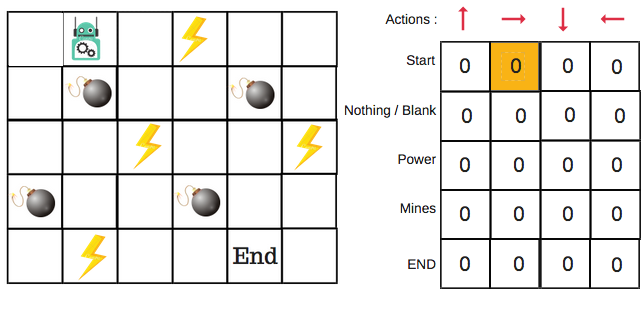
\includegraphics[width=0.7\linewidth]{tabular-table.png}}
    \caption{Ví dụ về tabular method}
    \label{fig:problem:tabular}
\end{figure}
\subsection{Huấn luyện mô hình học tăng cường sử dụng mạng neural}
Tuy nhiên với những bài toán phức tạp có không gian trạng thái vô cùng lớn hoặc có thể là vô hạn như không gian liên tục, thì cách tiếp cận theo kiểu tabular methods sẽ không phù hợp. 
Thay vào đó bằng cách sử dụng mô hình và ý tưởng của mạng neural, ta có thể ước lượng được một policy tối ưu. Thay vì nhìn vào bảng để tra cứu ta coi policy tương tự như một mạng neural với đầu vào là trạng thái hiện tại của environment và đầu ra chính là hành động tương ứng với trạng thái đó. 

Để đơn giản quá trình xem xét bài toán và huấn luyện trong đồ án này tôi sẽ tập trung vào việc sử dụng ANN đơn giản là mạng neural lan truyền thẳng (thuật ngữ gốc: \emph{feed-forward neural network}) để học tập bộ tham số cho policy. 

Các bước xây dựng mô hình học như sau:
\begin{enumerate}
    \item Sử dụng hàm policy hiện tại để tạo ra một chu trình: $S_{0}, A_{0}, R_{1}, S_{1}, A_{1}, R_{2}, S_{2}, A_{2}, R_{3}, \dots$
    \item Từ chu trình này, tính toán giá trị của value function từ thời điểm bắt đầu: ($t=0$) $ G_{0} \doteq R_{1}+R_{2}+R_{3}+\cdots+R_{T}$
\end{enumerate}

Bộ tham số của một mạng policy sẽ bao gồm tập các \textbf{tham số} và \textbf{độ lệch} ($W_1, b_1, W_2, b_2, ...$). Các tham số này sẽ được tối ưu sao cho cực đại hóa giá trị mục tiêu $G_k$ tại từng thời điểm $t=k$.
\begin{equation}
    maximize_{\{W_1, b_1, W_2, b_2...\}} G_k
\end{equation}

% \subsection{Các tiếp cận tiến hóa trong huấn luyện mô hình học tăng cường}
% Có rất nhiều cách để sử dụng EA để khám phá không gian policy trong RL\cite{moriarty1999earl}, trong phần này tôi sẽ mô tả một phương pháp đơn giản để biểu diễn không gian chung policy trong RL. Đó là phương pháp sử dụng một nhiễm sắc thể đơn để biểu diễn một policy với các gen là trọng số của mạng Neural như trong hình \ref{fig:problem:policy}. 
\begin{figure}[ht]
    \centering
    \fbox{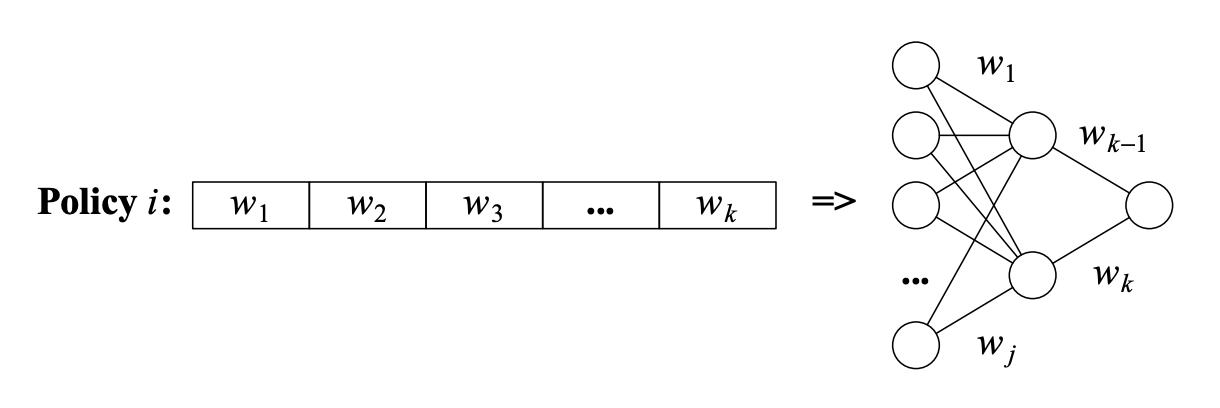
\includegraphics[width=0.7\linewidth]{policy.png}}
    \caption{Cách biểu diễn policy đơn giản bao gồm các trọng số của mạng neural.}
    \label{fig:problem:policy}
\end{figure}
Một mô hình mạng policy được biểu diễn bởi một cấu trúc mạng $H=(h_1,h_2,...h_k)$ có số lớp là $L$ ta sẽ thực hiện tính toán kích thước của không gian chung tương ứng với cấu trúc mạng này:
\begin{align}
    D_{chung} = \sum_{l={1,...L}}(h_{l-1}\cdot h_l + h_l)
\end{align}

Các tham số của mạng sẽ được mã hóa lần lượt vào không gian chung này. Khi cần đánh giá fitness trên một biểu cá thể ta sẽ giải mã từ nhiễm sắc thể về các bộ tham số $w$ và độ lệch $b$ tương ứng để tính tổng phần thưởng thu được với bộ tham số này.

% Quá trình mã hóa và giải mã này được biểu diễn trong hình \ref{fig:problem:policy-decode}.

% Để tìm kiếm tập tham số tối ưu cho \emph{policy}, EA lưu trữ một quần thể với nhiều nhiễm sắc thể khác nhau. Mỗi nhiễm sắc thể trong quần thể có thể được giải mã thành các tham số cho mạng Nơ-ron của \emph{policy}. 

% Tuy nhiên việc giải mã còn phụ thuộc vào ta mã hóa một nhiễm sắc thể như thế nào. Có nhiều phương pháp mã hóa nhiễm sắc thể có thể sử dụng, đa phần chúng được chia thành 2 nhóm:
% \begin{enumerate}
%     \item Mã hóa nhiễm sắc thể gián tiếp nghĩa là chỉ có một số thành phần, cấu trúc bên trong nhiễm sắc thể sẽ tạo lên toàn mạng. 
%     \item Mã hóa nhiễm sắc thể trực tiếp nghĩa là toàn bộ các thành phần, cấu trúc bên trong nhiễm sắc thể sẽ cấu thành lên mạng Nơ-ron.
% \end{enumerate}
